

\documentclass[10pt, conference, compsocconf]{IEEEtran}

\usepackage{multirow}
\usepackage{subfigure}
\usepackage{graphicx}
\usepackage{graphics}
\usepackage{rotating}
%\usepackage{times}
%\usepackage[centertags]{amsmath}
%\usepackage{amsfonts}
%\usepackage{amssymb}
%\usepackage{amsthm}
%\usepackage{glossary}
%\usepackage{epsfig}
%\usepackage{algorithm}
%\usepackage{algorithmic}






% *** GRAPHICS RELATED PACKAGES ***
%
\ifCLASSINFOpdf
  % \usepackage[pdftex]{graphicx}
  % declare the path(s) where your graphic files are
  % \graphicspath{{../pdf/}{../jpeg/}}
  % and their extensions so you won't have to specify these with
  % every instance of \includegraphics
  % \DeclareGraphicsExtensions{.pdf,.jpeg,.png}
\else
  % or other class option (dvipsone, dvipdf, if not using dvips). graphicx
  % will default to the driver specified in the system graphics.cfg if no
  % driver is specified.
  % \usepackage[dvips]{graphicx}
  % declare the path(s) where your graphic files are
  % \graphicspath{{../eps/}}
  % and their extensions so you won't have to specify these with
  % every instance of \includegraphics
  % \DeclareGraphicsExtensions{.eps}
\fi

% correct bad hyphenation here
\hyphenation{Dirt Spot Sweeping Random Strategy}


\begin{document}
%
% paper title
% can use linebreaks \\ within to get better formatting as desired
\title{Dirt Spot Sweeping Random Strategy}


% author names and affiliations
% use a multiple column layout for up to two different
% affiliations

\author{\IEEEauthorblockN{Mian Asbat Ahmad}
\IEEEauthorblockA{Department of Computer Science\\
The University of York\\
York, United Kingdom\\
ma@cs.york.ac.uk}
\and
\IEEEauthorblockN{Manuel Oriol}
\IEEEauthorblockA{Department of Computer Science\\
The University of York\\
York, United Kingdom\\
manuel@cs.york.ac.uk}
}


% make the title area
\maketitle


\begin{abstract}

All  the  strategies  used in the automated software testing tools for finding faults in the given Software Under Test (SUT) aim  to  detect  maximum  number  of  faults  in  minimum  amount of time. This can be achieved if test strategy selects more faults targeted test cases from the input domain for the given SUT, however, it is not that easy to produce such targeted test cases because each system has its own requirements and functionality. \\   

In this article an enhanced and improved form of automated random testing, called Dirt Spot Sweeping Random (DSSR) strategy, is introduced. DSSR strategy  is  a  new  strategy  that  not  only  combines  ordinary  random  strategy  and  random  plus strategy  to  achieve their combined benefits but additionally sweeps the dirt spots (Faulty patterns) in the program code for faults. It is based on two intuitions, first is that test values in boundaries of equivalence partition  are  interesting,  using  these  test  values  in  isolation  can  detect  new  faults  in  the  system, which produce high impact on test results while second is that faults reside in block and strip pattern inside the input domain of the program therefore when a fault is found, using neighbouring values of the fault finding value  can  reveal  more  faults  quickly  which  consequently  increases  the  test performance. \\

DSSR  strategy  is  implemented  in  an  automated  random  testing  tool  called  York Extensible Testing Infrastructure (YETI). Using this tool several experiments were performed on two groups  of  classes.  First  group  was  seeded  with  errors  of  block/strip  nature  while  the  second  group was  more  generalized  containing  classes  from  the  database  of  various  Java  systems  maintained  in Qualitas Corpus. Performance was measured in terms of number of faults found in specific number of  test  cases by each strategy.  Experimental  results  of  group  1  showed  that  DSSR  strategy  is  up  to  30\%  better  than random  and  random  plus  because  it  effectively  sweeps  the  blocks/strips.  In  the  second  group random  plus  was  better  followed  by DSSR  and  then pure  random  strategy. It  is  because  that  there were no block/strip patterns in the second group code.

\end{abstract}

\begin{IEEEkeywords}

random testing; automated testing; YETI; DSSR; test strategy;

\end{IEEEkeywords}


\IEEEpeerreviewmaketitle

\section{Introduction}
% no \IEEEPARstart
In the present era, the use of software is obligatory for the stability, dignity and  prosperity of a country. The basic purpose of any software is to serve the man kind in a  precise, simple, efficient, reliable and robust manner but all these features are not easily achievable. To incorporate these features in a software, it has to pass through many stages of quality control and testing particularly in its development phase. Limited software development time with strict deadlines for production make the target even harder to achieve. Therefore it is always desirable to have a quick yet efficient testing procedure to ensure high quality in minimum possible time. To meet these challenges researchers are trying their best to develop new and improve the existing techniques of software testing for finding more faults with fewer number of test cases. Random testing is one such technique which is highly efficient, consumes less computation power and can be easily automated.\\

Random testing is a black-box testing technique in which the System Under Test (SUT) is executed against randomly selected test data. Test results obtained are compared against the oracle defined using SUT specifications in the form of contracts or assertions. In the absence of contracts/assertions the exceptions defined by the programming language in which the program is developed is used as test oracle. According to Beizer, \cite{Beizer1990} software performance is directly dependant on the combination of two main factors that include correctness and robustness. Correctness is the expected behaviour of the software based on its specifications while robustness is the behaviour of the software which is not defined in its specifications. Since random testing generates test data randomly without any specific pattern therefore it effectively test the performace of software by evaluating it for both correctness and robustness. Because of its black-box testing nature it is particularly effective in testing softwares where the developers wants to keep the source code secret \cite{Chen2010}. The generation of random test data is comparatively cheap and does not require too much intellectual and computation efforts \cite{Ciupa2009}, \cite{Ciupa2008}. It is mainly for this reason that various researchers have recommended this strategy for incorporation in automatic testing tools \cite{Ciupa2008a}. YETI \cite{Oriol2010a}, \cite{Oriol2010}, AutoTest \cite{Leitner2007}, \cite{Ciupa2007}, QuickCheck \cite{Claessen2000}, Randoop \cite{Pacheco2007}, JArtage \cite{Oriat2004} are a few of the most common automated testing tools based on random strategy.\\

In the past random testing went through some controversies in terms of performance. The efficiency of random testing was made suspicious with the intuitive statement of Myers \cite{Myers2004} who termed random testing as one of the poorest methods for software testing, however in science there is no substitute for experimental analysis and later on various experiments performed by different researchers \cite{Ciupa2007}, \cite{Duran1981}, \cite{Duran1984}, \cite{Hamlet1994} and \cite{Ntafos2001}  experimentally proved that random testing is simple to implement, cost effective, highly efficient and free from human bias compared to its rival techniques. \\

The researchers found that the performance of random testing can be further increased by slightly altering the technique of test case selection. In adaptive random testing, Chen et al.  \cite{Chen2008} found that the performance of random testing increases by up to 50\% when test input is selected evenly which is spread across the whole input domain. Similarly Restricted Random Testing \cite{Chan2002}, Feedback directed Random Test Generation \cite{Pacheco2007a}, Mirror Adaptive Random Testing \cite{Chen2003} and Quasi Random Testing \cite{Chen2005} also stressed on the need of test case selection covering whole of the input domain for better results. \\


\begin{figure}[htp]
\centering
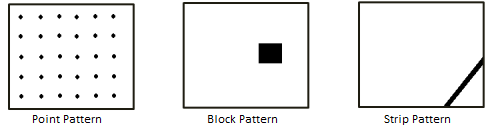
\includegraphics[width=8cm,height=2.5cm]{figures/ART_Patterns.png}
\caption{Failure patterns across input domain \cite{Chen2006}}
\label{fig:patterns}
\end{figure}

Chen et al. \cite{Chen2008} further found that there are patterns of failure causing inputs across the input domain. They divided these patterns into three types called block, point and strip patterns. They also said that a strategy can get more chances of hitting these fault patterns if test cases far away from each other are selected. Various other researchers \cite{Chan2002}, \cite{Chen2003} and \cite{Chen2005} also tried to generate test cases further away from one another targeting these patterns to achieve higher performance. Failure patterns are illustrated in Figure \ref{fig:patterns}.\\


Random plus \cite{Leitner2007} is an updated version of the pure random strategy. It is a modified form of random strategy that uses some special pre-defined values which can be simple border values or values that have high tendency of finding faults in the SUT. Boundary values \cite{Beizer1990} are the values on the start, end and middle of a particular type. For instance,  Integer.MIN\_VALUE -1, Integer.MIN\_VALUE, Integer.MIN\_VALUE +1, -3, -2, -1, 0, 1, 2, 3, Integer.MAX\_VALUE -1, Integer.MAX\_VALUE, Integer.MAX\_VALUE + 1, can be considered as border values for Integer data type. Similarly the tester might also add some other special values that he consider effective in finding faults for the current SUT. For example, if a program under test has a loop from 1 to 100 then the tester can add 100, 101, 99, 51, 50, 49, -1, 0 and 1 etc to the pre-defined list of special values in order to be selected for a test. This list of interesting values has slightly high priority than selection of random values because of its more relevance and high chances of finding faults. It is found that these special values have high impact on the results particularly detecting problems in specifications \cite{Ciupa2008}.\\

The rest of this paper is organized as follows. The sections, II to X, describe Dirt Spot Sweeping Random (DSSR) strategy, Implementation of DSSR strategy, Experimental setup and analysis, Evaluation of DSSR strategy, Experimental results, Unique faults found by DSSR strategy, discussion, conclusion and future work respectively.\\ 
%\pagenumbering{arabic}
%\setcounter{page}{1}


\section{Dirt Spot Sweeping Random Strategy}

Dirt Spot Sweeping Random (DSSR) strategy is a new random test strategy developed during this study. DSSR strategy is the combination of two existing strategies i.e. pure random and random plus with the addition of one new strategy called spot sweeping. It is based on two intuitions. Intuition No. 1 is that boundaries have interesting values and using these values in isolation can provide high impact on test results, while intuition No. 2 is that faults can reside in block and strip pattern thus using neighbouring values of the fault finding value can lead us to the next fault in the same block or strip. This increases the performance of the test strategy in terms of executing fewer number of test cases with more number of faults. It is to be noted that random plus test strategy add border values before the test starts whereas spot sweeping test strategy add fault finding values and its neighbouring values to the list of interesting values at run time when they are found during testing. We can also say that in random plus the list of interesting values remain static/constant whereas in DSSR strategy the list of interesting values is dynamic and changes during the execution of the program.\\

Initially, the DSSR strategy was not utilizing the boundary values of random plus strategy and the list of interesting values was empty at the start of the test. Therefore, in the earlier version, the test had to start with random testing and once the fault was found in the system, DSSR strategy would transfer the fault finding test value and the surrounding values to the list of interesting values. In this way the list of interesting values is populated and the strategy now looks for interesting values in the list before trying to get any arbitrary random value. The bottle-neck in this strategy was that DSSR strategy had to wait for the random testing to find the fault in the system. This bottle-neck was removed by introducing border values in DSSR strategy while keeping the remaining process the same. In updated version the border values are added to the list of interesting values before the test starts thus from the beginning of the test the system not only selects purely random values but also checks for values from boundary values, which increases the fault finding chances and consequently add more values to the list of interesting values \cite{Kaner2004}.\\

\begin{figure}[htp]
\centering
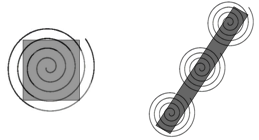
\includegraphics[width=8cm,height=3cm]{figures/block2.png}
\caption{DSSR covering block and strip pattern}
\label{fig:block2}
\end{figure}

Figure \ref{fig:block2} shows how DSSR strategy explores the faults residing in the block and strip patterns of a program. The testing process starts with pure random and random plus strategy. When the fault is found the DSSR strategy adds the test input value which causes the fault and its neighbouring values to the list of interesting values. Now if the fault is positioned on the block or strip pattern then the neighbouring values will explore the whole block and strip pattern by finding new faults and adding its neighbours values untill all the faults in that block or strip are identified. The faults coverage from the block and strip pattern is shown in spiral form because first fault will lead to second, second to third and will continue untill it ends. But if that fault is positioned on the point pattern then the added values will not be very effective because point pattern is only an arbitrary point in the whole input domain containing a single fault.\\

Before its implementation and evaluation, the following research questions about the DSSR strategy were formulated and subsequently addressed:\\
\begin{enumerate}

\item To get highly efficient algorithm to cope with the combination of strategies including pure random, random plus and spot sweeping which further populate the list of interesting values with fault finding value and its neighbouring values to provide more relevant test values to the Test engine. \\

\item To get high number of unique faults because according to Chen et al. \cite{Chen2006} most of the faults reside in block and strip pattern which is efficiently covered by DSSR strategy. \\

\item To get  low number of unique faults and high number of similar faults because the faults in the same block and strip pattern across the program might be of similar nature.\\

\item  Not to get any particular improvement if the program don't contain any block or strip pattern but contain only point pattern.\\

\item  DSSR strategy might consume more time to execute the same set of test cases than random and random plus strategy because of extra processing when analyzing values at runtime, transferring them to the list of interesting values and selecting appropriate test value from the list when required during test.\\



\end{enumerate}

\subsection{Structure of Dirt Spot Sweeping Random Strategy}

\hspace{10 mm}The DSSR strategy is explained with the help of flow-chart in Figure \ref{fig:Working_DSSS}. In this process the DSSR strategy continuously track the number of faults during the exection of the test session. To keep the system fast this tracking is done in a very effective way with 0 or minimum overhead \cite{Leitner2009}. Execution of test is performed normally untill a fault is found in the SUT. When a fault is found the program not only copy the value that lead to the fault, but also copy its surrounding values to the variable list of interesting values. From the flow-chart you can see that if the fault finding value is of primitive type then the test strategy DSSR finds the type of that primitive value and add values only of that particular type to the interesting values list. Addition of these values increases the size of the list of interesting values which provide relevant test data for the remaining test session and the new generated test cases are more targeted towards finding new faults in the given SUT.\\

\begin{figure}[htp]
\centering
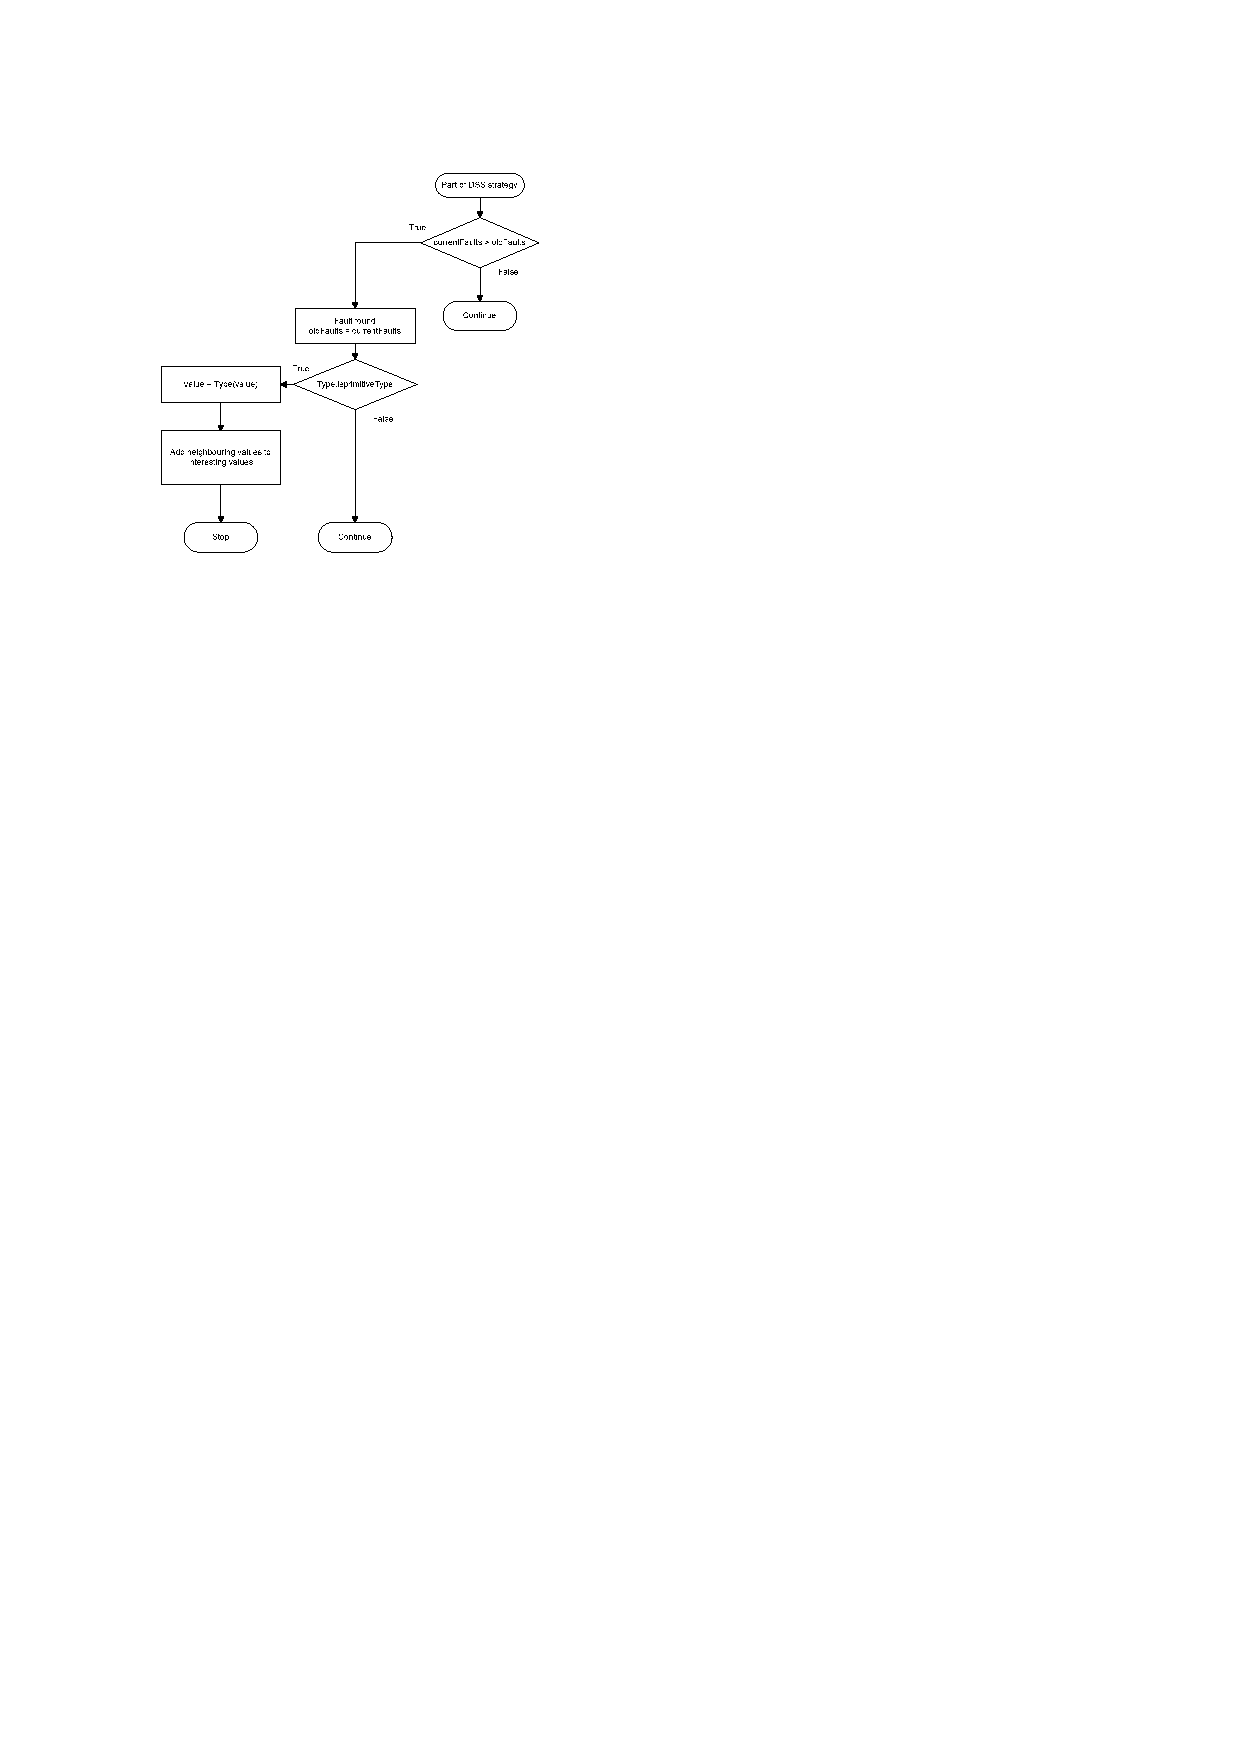
\includegraphics[width=8.5cm,height=12cm]{figures/flowchart1.pdf}
\caption{Working mechanism of DSSR Strategy}
\label{fig:Working_DSSS}
\end{figure}

Border values and other special values that have high tendency of finding faults in the SUT are added to the list by random plus strategy (extention of pure random) prior to the start of test session where as to sweep the failure pattern, fault value and fault surrounding values are added at run time after a fault is found. Table \ref{table:addvalues} contains the values that are added to the list of interesting values when a fault is found. The test value is represented by X where X can be int, double, float, long, byte, short, char and String. All values are converted to their respective types before adding to the list of interesting values and vice versa.

\begin{table}[ht]
\scriptsize
\caption{Neighbouring values for primitive types and String} % title of Table
\centering % used for centering table
\begin{tabular}{| l | l |} % centered columns (4 columns)
\hline\hline %inserts double horizontal lines
Type & Values to be added\\ [0.5ex] % inserts table
%heading
\hline % inserts single horizontal line
\multirow{3}{*}{X is int, double, float, long, byte short and char} & X \\ % inserting body of the table

&[[X-3 , X-1]] \\
&[[X+1 , X+3]]\\
\hline
\multirow{8}{*}{X is String} & X\\ % inserting body of the table

& X + ``  "\\ % inserting body of the table
& ``  " + X \\ % inserting body of the table
& X.toUpperCase() \\
& X.toLowerCase() \\
& X.trim() \\
& X.substring(2) \\
& X.substring(1, X.length() - 1) \\[1ex]
\hline
\hline %inserts single line
\end{tabular}
\label{table:addvalues} % is used to refer this table in the text
\end{table}


\subsection{Motivating Example}
% no \IEEEPARstart
To further clarify the working mechanism of DSSR strategy we have written the following simple program which is planted with atleast three faults. The first one is division by zero exception while the other two are in the form of assertion statements at line 3 and 4.  Below we describe how DSSR strategy will perform execution when the following class is supplied for testing.\\

\noindent
/ \textasteriskcentered \textasteriskcentered \\*
\textasteriskcentered   ~ Calculate square of given number and verify results. \\*
\textasteriskcentered   ~ Code contain 3 faults.\\*
\textasteriskcentered   ~ @author (Mian and Manuel) \\* 
\textasteriskcentered   ~ @version (1.1, 11/11/11)\\*
\textasteriskcentered / \\*

public class Math \{\\

\hspace{7mm} public void calc ( int a) \{\\

//Square the value and assign it to result.\\*

1.\hspace{12mm} int result1 = a * a;\\*

2. \hspace{12mm}int result2 = result1 / a;\\*

//To check that the value of result is positive.\\*

3.\hspace{12mm} assert result1 $>$ a;\\*

//To check that the revert of result is the received value.\\*

4. \hspace{12mm}assert Math.sqrt(result1) = a;\\*



\hspace{7mm}\}  \\*

\}\\*

\hspace{10 mm}From the above code we can see that only one primitive type is used which is ``int" and we also know that for ``int" beside other values we have special pre-defined values including 0, Integer.MAX\_VALUE and Integer.MIN\_VALUE in the list of interesting values. Now on starting the test we will immediately find all the faults in the following order using DSSR strategy where as pure random and random plus strategy on the other hand will try randomly to find each fault even if the first fault is found which is very closed to the second one.\\*



\textbf{Fault 1:} The DSSR strategy might select value 0 for variable ``a"  in the first test case because 0 is available in the list of interesting values and therefore its priority for selection is higher than other values. This will cause Java to generate division by zero from line 2 because any integer divided by zero is infinity.\\*

\textbf{Fault 2:} When DSSR strategy catch the failure it will add this and the surrounding values to the list of interesting values which includes 0, 1, 2, 3 and -1, -2, -3. Now for the second test case DSSR strategy may pick -3 as a test value and it will take us to our second fault where assertion no 2 (line 4) will fail because the square root of -3 will be +3 instead of the original supplied number -3.\\*

\textbf{Fault 3:} After a few test cases the DSSR strategy might select Integer.MAX\_VALUE for variable ``a" which is also available in the list of interesting values and it will lead us to our 3rd fault because result1 will not be able to store the square of Integer.MAX\_VALUE. Instead of the actual calculated square value Java will assign a negative value (Java language rule) to variable result1 which will lead to the violation of assertion 1 (line 3) and we will get our 3rd and final fault.\\*


From the above execution process we can understand that, in this example, pre-defined values including border values, fault finding values and its surrounding values lead us quickly to the available faults and in less number of tests as compared to pure random and random plus which randomly selects test values across the whole input domain in a traditional fashion.

\section{Implementation of DSSR strategy}

The DSSR strategy was implemented in YETI tool \cite{Oriol2011}. YETI is an automated random testing tool developed in Java. It is an open source tool capable of testing both procedural and object-oriented softwares. Its language-agnostic meta model enables it to test programs written in multiple languages including Java, C\#, JML and .Net. The core features of YETI includes easy extensibility for future growth, speed of up to one million calls per minute on java code, real time logging, real time GUI support, ability to test programs using multiple strategies and auto generation of test report at the end of the test session. A number of hitherto faults have successfully been found by YETI in various production softwares. \\

YETI can be divided into three main sections including core infrastructure, language-specific bindings and strategies. The core infrastructure represents routines, a group of types and a pool of specific type objects. The  language specific bindings contain the code to make the call and process the results. The strategies section defines the way to select the class/module to test random selection of routine/method from the given module and get instances of the required type during testing. DSSR strategy is also added to the strategies section of YETI tool with the class name YetiDSSRStrategy. It is extention of YetiRandomStrategy which in itself is extention of an abstract class YetiStrategy. The class hierarchy is shown in Figure \ref{fig:hierarchyofDSSR}.\\

\begin{figure}[htp]
\centering
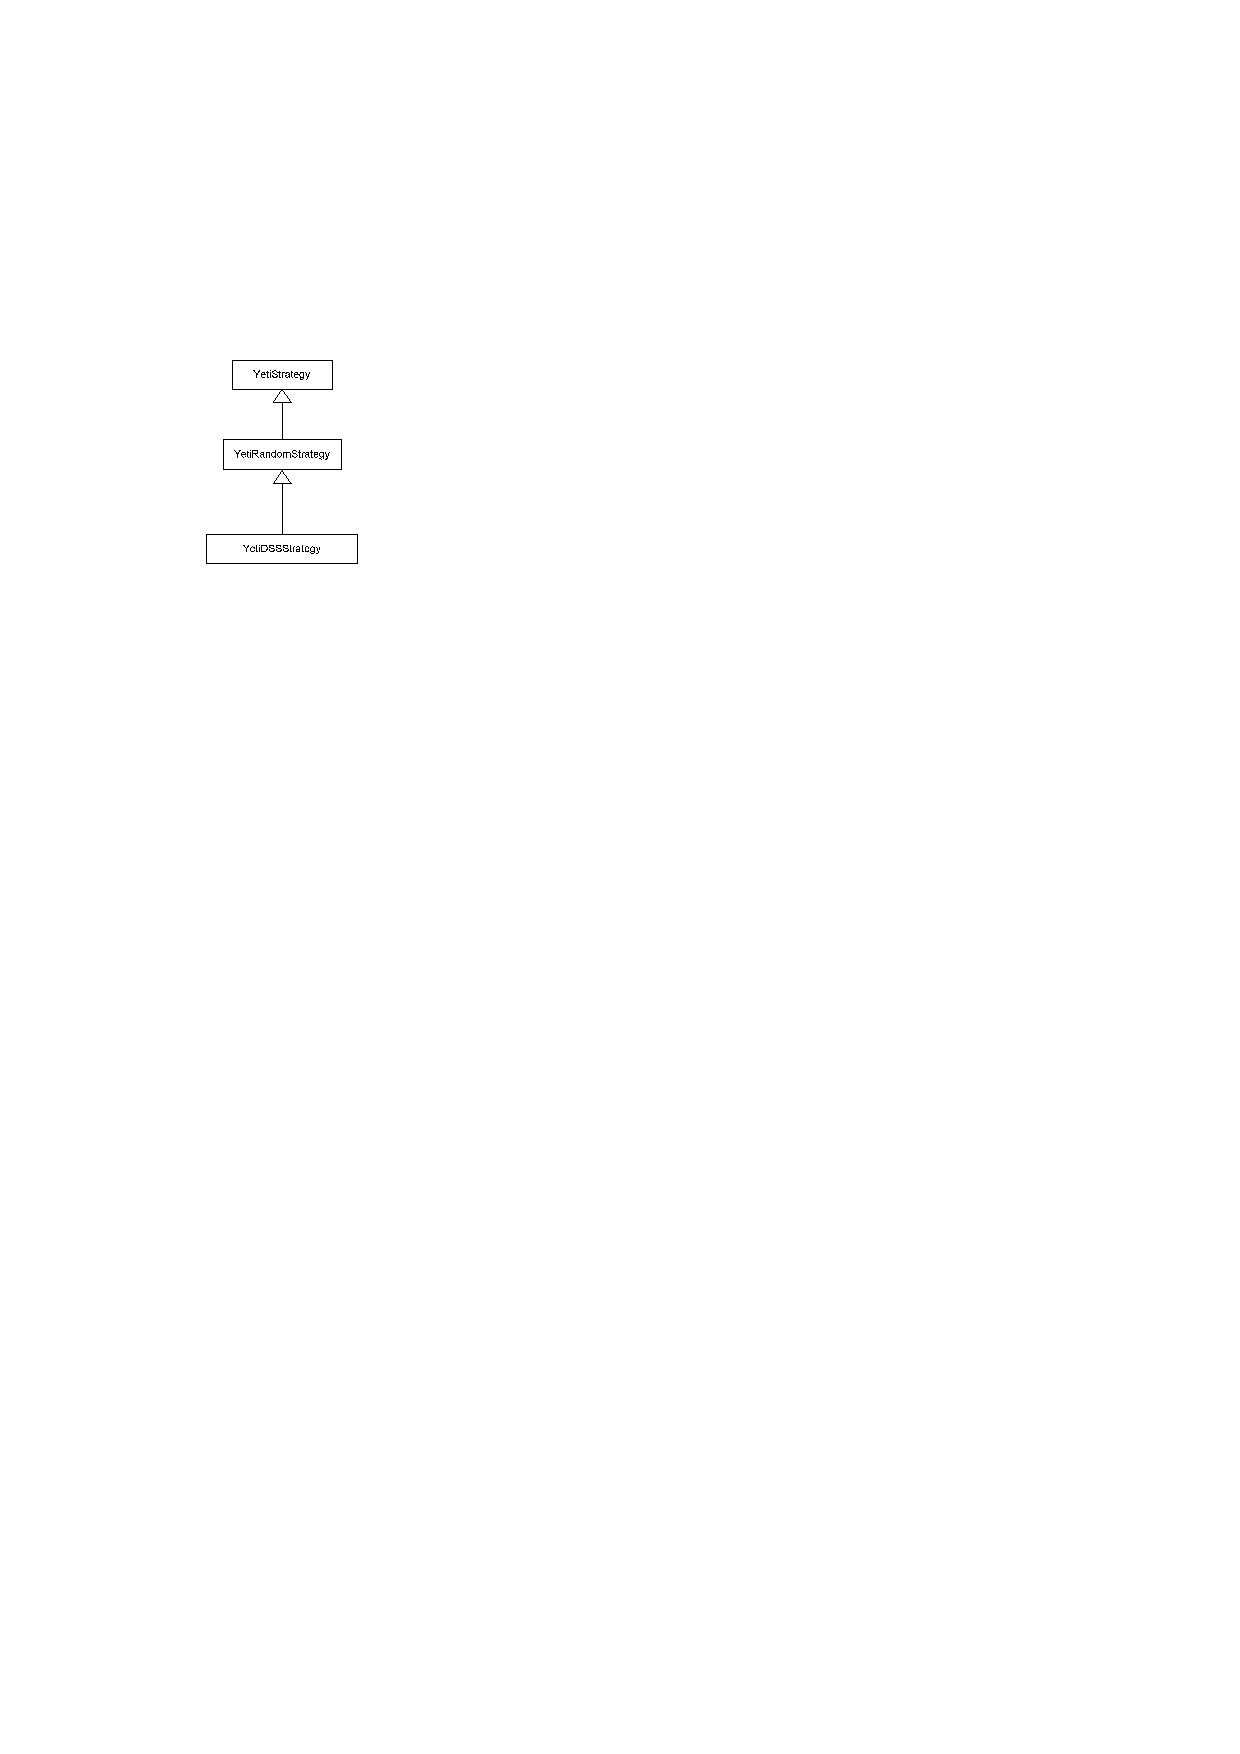
\includegraphics[width=5cm,height=7cm]{figures/hierarchy.pdf}
\caption{Class Hierarchy of DSSR in YETI}
\label{fig:hierarchyofDSSR}
\end{figure}


If no particular strategy is defined during test initialization then YETI will use its default random plus strategy in which the user can control the probability of null values and the percentage of newly created objects. Both probabilities are set to 10\% by default. \\

YETI also provide an interactive Graphical User Interface (GUI) where a user can see the progress of the current test in real time. Besides GUI, YETI also provides extensive logs of the test session which are very helpful in fault tracking. For more details about YETI see references \cite{Oriol2010a} and \cite{Oriol2010}.

\section{Experimental setup and Analysis}

To evaluate the performance of DSSR strategy we performed several experiments. A total of 15 classes were rigorously tested where 5 of the classes were written specifically to evaluate the DSSR strategy while 10 classes were selected randomly from java.lang and java.util packages of Java Development Kit (JDK). Since the performance of random strategy cannot be evaluated from a few tests because of its random behavior therefore each class was tested 10 times by pure random and DSSR strategy. The GUI of YETI show multiple real time graphs including one for unique failures. There is also a handy option in YETI front end where user can right click any of the graph and save the data about it in a text file. The same option was utilized to store the unique failures found in each experiment for further analysis. Another feature called "Interesting value injection probability" gives control on the selection of test data either from the list of interesting values or randomly from the available pool. YETI also allow user to set a specific number of calls for which values should be selected from the list of interesting values. For all our experiments the interesting value injection probability was set to 0.1, which means that 10\% of the test values will be selected from the list of interesting values while remaining 90\% of the values will be selected randomly.\\

For DSSR strategy the probability to select values from the list of interesting values and null values were kept constant for all the experiments. Experiments were divided into two groups. In the first group of experiments our own written error seeded classes were tested while in the second group random classes from java.util and java.lang packages were selected. Each class of both the groups were tested 10 times by both DSSR and random strategy. The total number of experiments were 10 x 10 x 15 = 1500. The number of tests for each class in group 1 were kept 10,000 so the total tests are 10,000 x 10 x 10 x 5 = 5,000,000.  For group 2 the number of tests were decreased to 500 so that the total tests conducted in group 2 were 500 x 10 x 10 x 10 = 500,000 tests. The use of error seeded programs made it possible to assess the two strategies objectively by measuring the total number of faults found and the test execution duration by each strategy. The automated oracle used for all experiments was the defined exception of the language because of the absence of the contracts and assertions in the code under test.\\

Commands for executing the experiments using pure random and DSSR strategies are as follows. Since pure random is the default strategy for testing in YETI therefore there is no need to mention that strategy in the command.\\*

\begin{itemize}

\item java yeti.Yeti -java -testModules=java.lang.String -nTests=10000 -nologs -gui\\*

\item java yeti.Yeti -java -testModules=java.lang.String -nTests=10000 -nologs -gui -DSSR\\*

\end{itemize}

Various options used in the above commands have the following meanings:\\*
\textbf{yeti.Yeti} represents the package name (yeti) and the main class (YETI).\\*
\textbf{-java} is used to show that the program under test is written in Java language.\\*
\textbf{-testModules} points to the system under test, which is String in this case.\\*
\textbf{-nTests} is used to execute specified number of test calls in that session, which is 10,000 and 500 for both of the strategies.\\*
\textbf{-nologs} is used so that logs are not printed on the screen during test execution. This option is enabled to decrease extra load on the processor.\\*
\textbf{-gui} is used to show the real time test results in Graphical User Interface on display.\\*
\textbf{-DSSR} is used to select the Dirt Spot Sweeping Random strategy for the current test session.\\*

All tests were performed using 64-bit Microsoft Windows 7 Enterprise Service Pack 1 running on Intel(R) Core(TM)2 Duo CPU E8400 @ 3.00GHz with 4.00 GB RAM. Furthermore, Java(SE) Runtime Environment [Version 6.1.7601] was used.\\

Each test is explained with the help of a table and figure. Table \ref{table:five}, \ref{table:tena} and \ref{table:tenb} present the results of the tests performed using random and DSSR strategy while figure \ref{fig:Result1} and \ref{fig:Result2} depict the summary of all the tests.



\subsection{Performance criteria used in the experiments}
Various measures including F-measure, P-measure and E-measure have been used by researchers to find the effectiveness of the random test strategy. E-measure (Expected number of failures detected) and P-measure (Probability of detecting atleast one failure) received criticism from researchers \cite{Chen2008} and are not considered effective techniqes for measuring efficiency of test strategy. F-measure (Number of test cases used to find the first fault) used by researchers  \cite{Chen1996}, \cite{Chen2004} is quite well known and initially we used it in our experiments to calculate the efficiency. After a few experiments we came to know that this was not the right choice because in some experiments the first strategy found first fault quickly than the second strategy but after the complete test session the first strategy found lower number of total faults than the second strategy. In our view it is not fair to prefer a strategy only because it found the first fault better without giving due consideration to the total number of faults. Moreover, for random testing F-measure is quite unpredictable because its value can be easily increased by adding more narrow conditional statements in the SUT. For example in the following program it is difficult for random testing to generate the exact number (3.3338) quickly and therefore the F-measure will be high.\\

\{ \\*   

\hspace{07 mm}if ( (value $>$  3.3337) \&\& (value $<$ 3.3339) )\\*

\hspace{07 mm}\{ 10/0 \} \\* 

\} \\*

Therefore in all our experiments performance of the strategy was measured in terms of finding maximum number of faults in a particular number of test calls  \cite{Ciupa2007}, \cite{Pacheco2007a}, \cite{Ciupa2008b} which in our case was set to 10,000 and 500 calls per class. The number of test calls was kept constant for both pure random and DSSR strategy in all the experiments. This measurement was found effective because it clearly measured the performance of the strategy when all the other factors were kept constant.\\



%\pagenumbering{arabic}
%\setcounter{page}{1}

\section{Evaluation of DSSR strategy}
To evaluate the new DSSR strategy in terms of performance we performed extensive experiments. To get a clear view of its performance we determined the comparative performance of DSSR strategy with pure random strategy by applying them to similar systems under identical conditions. Performance was measured in terms of: the ability of a strategy to find maximum number of faults in a fixed number of tests and the time taken by each strategy to execute 10,000 and 500 tests for group1 and group2 respectively. In our experiments we gave due weightage to the number of faults as well as the time of execution because a strategy might be good in finding higher number of faults but may require more time to find these faults, thus not considered satisfactory in the field where emphasis is on speedy and accurate results. The number of tests were kept constant at 10,000 and 500 to get a fair competition among the two strategies otherwise both the strategies were capable of finding all the faults in the given SUT if the number of tests were increased to a reasonably higher level. Additional time taken to execute the test by each strategy was given due consideration in order to determine the number of test cases in a given time irrespective of the number of faults. 

\section{Results}


\begin{table}[ht]
\caption{Test results of 5 classes from java package. Each class is tested 10 times by both random and DSSR strategy.fs} % title of Table
\centering % used for centering table
\begin{tabular}{| c | c | c | c | c | c | c | c | c | c | c |} % centered columns (4 columns)
\hline\hline %inserts double horizontal lines
 \begin{sideways} Serial Number \end{sideways} &  \begin{sideways} y.t.Faulty1 by Random \end{sideways} &  \begin{sideways} y.t.Faulty1 by DSSR \end{sideways} &  \begin{sideways} y.t.Faulty2 by Random \end{sideways} &  \begin{sideways} y.t.Faulty2 by DSSR \end{sideways} & \begin{sideways} y.t.Faulty3 by Random \end{sideways} &  \begin{sideways}y.t.Faulty3 by DSSR \end{sideways} &  \begin{sideways}y.t.Faulty4 by Random \end{sideways} &  \begin{sideways} y.t.Faulty4 by DSSR \end{sideways} &  \begin{sideways} y.t.Faulty5 by Random \end{sideways} &  \begin{sideways} y.t.Faulty5 by DSSR \end{sideways} \\ [1ex] % inserts table
%heading
\hline  % inserts single horizontal line
1 & 1 & 2 & 0 & 2 & 2 & 3 & 0 & 2 & 1 & 3 \\  % inserting body of 

2 & 1 & 2 & 0 & 2 & 1 & 3 & 1 & 2 & 1 & 3 \\

3 & 0 & 2 & 0 & 2 & 2 & 2 & 0 & 2 & 0 & 3 \\

4 & 1 & 2 & 0 & 2 & 1 & 2 & 1 & 2 & 1 & 2 \\

5 & 0 & 2 & 0 & 2 & 2 & 3 & 1 & 2 & 1 & 2 \\

6 & 0 & 2 & 0 & 2 & 2 & 3 & 1 & 2 & 1 & 2 \\

7 & 1 & 2 & 0 & 2 & 1 & 3 & 0 & 2 & 1 & 3 \\

8 & 1 & 1 & 0 & 2 & 1 & 3 & 1 & 1 & 2 & 3 \\

9 & 1 & 2 & 0 & 2 & 1 & 3 & 1 & 2 & 1 & 3 \\

10 & 1 & 2 & 0 & 2 & 2 & 3 & 1 & 2 & 1 & 3 \\  [1ex] % [1ex] adds vertical spacefs

\hline %inserts single line
\end{tabular}
\label{table:five} % is used to refer this table in the text
\end{table}


Experimental finding indicate that DSSR strategy performs up to 30 \% better than pure random strategy. In some cases pure random strategy is not able to find even a single fault where as DSSR strategy finds all the available faults in the given SUT. Results of the group 1 tests are given in Table \ref{table:five} and the same data is also represented by a box-plot graph given in Figure \ref{fig:Result1}.\\


After confirmation of the effectiveness of DSSR strategy from group 1 experiments we performed similar tests on 10 random classes from Java JDK in group 2. Results were not very different and DSSR strategy gave better performance as presented in Table \ref{table:tena} and \ref{table:tenb}.  The data is also represented in Figure \ref{fig:Result2} using box-plot graph.\\



\begin{figure}[htp]
\centering
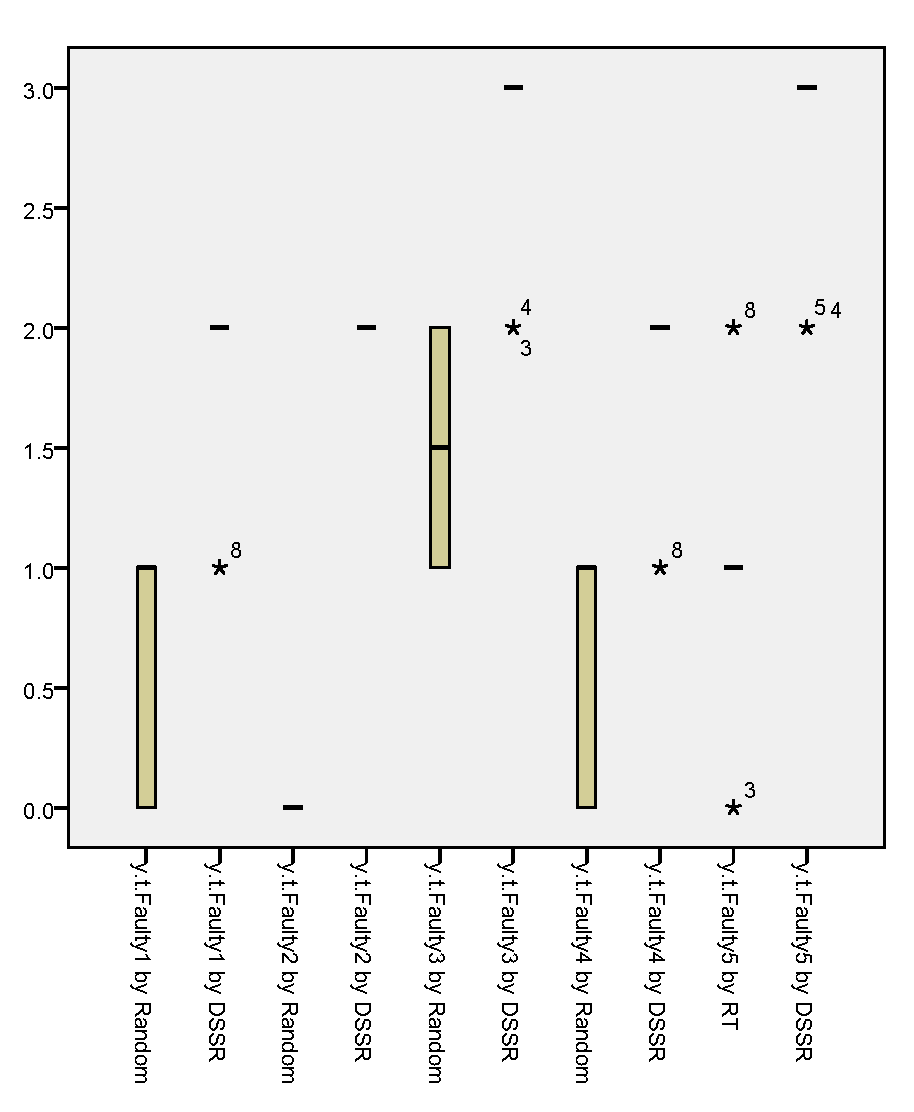
\includegraphics[width=7.5cm,height=9.5cm]{figures/owntests.png}
\caption{Test Results of 5 classes developed specially for DSSR analysis.}
\label{fig:Result1}
\end{figure}





\begin{table}[ht]
\caption{Test results of 10 classes from java package. Each class is tested 10 times by both random and DSSR strategy.fs} % title of Table
\centering % used for centering table
\begin{tabular}{| c | c | c | c | c | c | c | c | c | c | c |} % centered columns (4 columns)
\hline\hline %inserts double horizontal lines
 \begin{sideways} Serial Number \end{sideways} &  \begin{sideways} j.u.Character by Random \end{sideways} &  \begin{sideways} j.u.Character by DSSR \end{sideways} &  \begin{sideways} j.l.String by Random \end{sideways} &  \begin{sideways} j.l.String by DSSR \end{sideways} & \begin{sideways} j.u.Calendar by Random \end{sideways} &  \begin{sideways}j.u.Calender by DSSR \end{sideways} &  \begin{sideways}j.u.Scanner by Random \end{sideways} &  \begin{sideways} j.u.Scanner by DSSR \end{sideways} &  \begin{sideways} j.u.Properties by Random \end{sideways} &  \begin{sideways} j.u.Properties by DSSR \end{sideways}  \\ [0.5ex] % inserts table
%heading
\hline % inserts single horizontal line
1 & 11 & 13 & 8 & 8 & 4 & 4 & 41 & 41 & 13 & 14\\ % inserting body of 

2 & 13 & 12 & 8 & 8 & 3 & 3 & 39 & 42 & 12 & 13\\

3 & 12 & 14 & 6 & 7 & 3 & 4 & 41 & 41 & 12 & 13\\

4 & 12 & 12 & 7 & 8 & 4 & 4 & 39 & 43 & 12 & 13\\

5 & 11 & 12 & 8 & 7 & 4 & 4 & 38 & 42 & 13 & 13\\

6 & 13 & 11 & 6 & 7 & 3 & 4 & 38 & 39 & 12 & 14\\

7 & 11 & 12 & 7 & 8 & 4 & 4 & 39 & 39 & 12 & 14\\

8 & 13 & 12 & 7 & 8 & 4 & 4 & 41 & 42 & 13 & 13\\

9 & 12 & 12 & 8 & 8 & 4 & 4 & 37 & 42 & 13 & 13\\ 

10 & 13 & 14 & 4 & 7 & 4 & 4 & 40 & 41 & 14 & 13\\ [1ex] % [1ex] adds vertical spacefs

\hline %inserts single line

\end{tabular}
\label{table:tena} % is used to refer this table in the text
\end{table}


\begin{table}[ht]
\caption{Test results of 10 classes from java package. Each class is tested 10 times by both random and DSSR strategy.} % title of Table
\centering % used for centering table

\begin{tabular}{| c | c | c | c | c | c | c | c | c | c | c |} % centered columns (4 columns)
\hline\hline %inserts double horizontal lines
 \begin{sideways} Serial Number \end{sideways} & \begin{sideways} j.l.Thread by Random \end{sideways} &  \begin{sideways} j.l.Thread by DSSR \end{sideways} &  \begin{sideways} j.l.ProcessBuilder by Random \end{sideways} &  \begin{sideways} j.l.ProcessBuilder by DSSR \end{sideways} &  \begin{sideways} j.l.Double by Random \end{sideways} & \begin{sideways} j.l.Double by DSSR \end{sideways} &  \begin{sideways} j.l.ClassLoader by Random \end{sideways} &  \begin{sideways} j.l.ClassLoader by DSSR \end{sideways} & \begin{sideways} j.l.Character by Random \end{sideways} & \begin{sideways} j.l.Character by DSSR \end{sideways} \\ [0.5ex] % inserts table
%heading
\hline % inserts single horizontal line
1 & 4 & 4 & 29 & 28 & 9 & 9 & 17 & 18 & 25 & 34\\ % inserting body of 

2 & 4 & 4 & 30 & 25 & 10 & 8 & 26 & 27 & 24 & 35\\

3 & 4 & 4 & 30 & 31 & 7 & 17 & 26 & 29 & 28 & 34\\

4 & 4 & 4 & 28 & 29 & 8 & 8 & 16 & 26 & 23 & 35\\

5 & 4 & 4 & 32 & 34 & 7 & 1 & 11 & 22 & 26 & 33\\

6 & 4 & 4 & 31 & 31 & 8 & 9 & 12 & 18 & 26 & 34\\

7 & 4 & 4 & 28 & 26 & 10 & 8 & 8 & 10 & 29 & 37\\

8 & 4 & 4 & 29 & 27 & 9 & 8 & 14 & 21 & 24 & 31\\

9 & 4 & 4 & 28 & 30 & 14 & 11 & 07 & 29 & 25 & 32\\ 

10 & 4 & 4 & 30 & 33 & 11 & 10 & 26 & 20 & 26 & 38\\ [1ex] % [1ex] adds vertical spacefs

\hline %inserts single line
\end{tabular}
\label{table:tenb} % is used to refer this table in the text
\end{table}

\newpage

Figure \ref{fig:Result2} clearly depicts that DSSR strategy performs better than pure random strategy in group 2 experiments in almost all tests except java.lang.Thread where the test results are equal and both the strategies found the same number of faults. DSSR strategy particularly outperformed pure random strategy in java.lang.Character where it found 38 faults as compared to 29 faults found by pure random strategy.\\

\begin{figure}[htp]
\centering
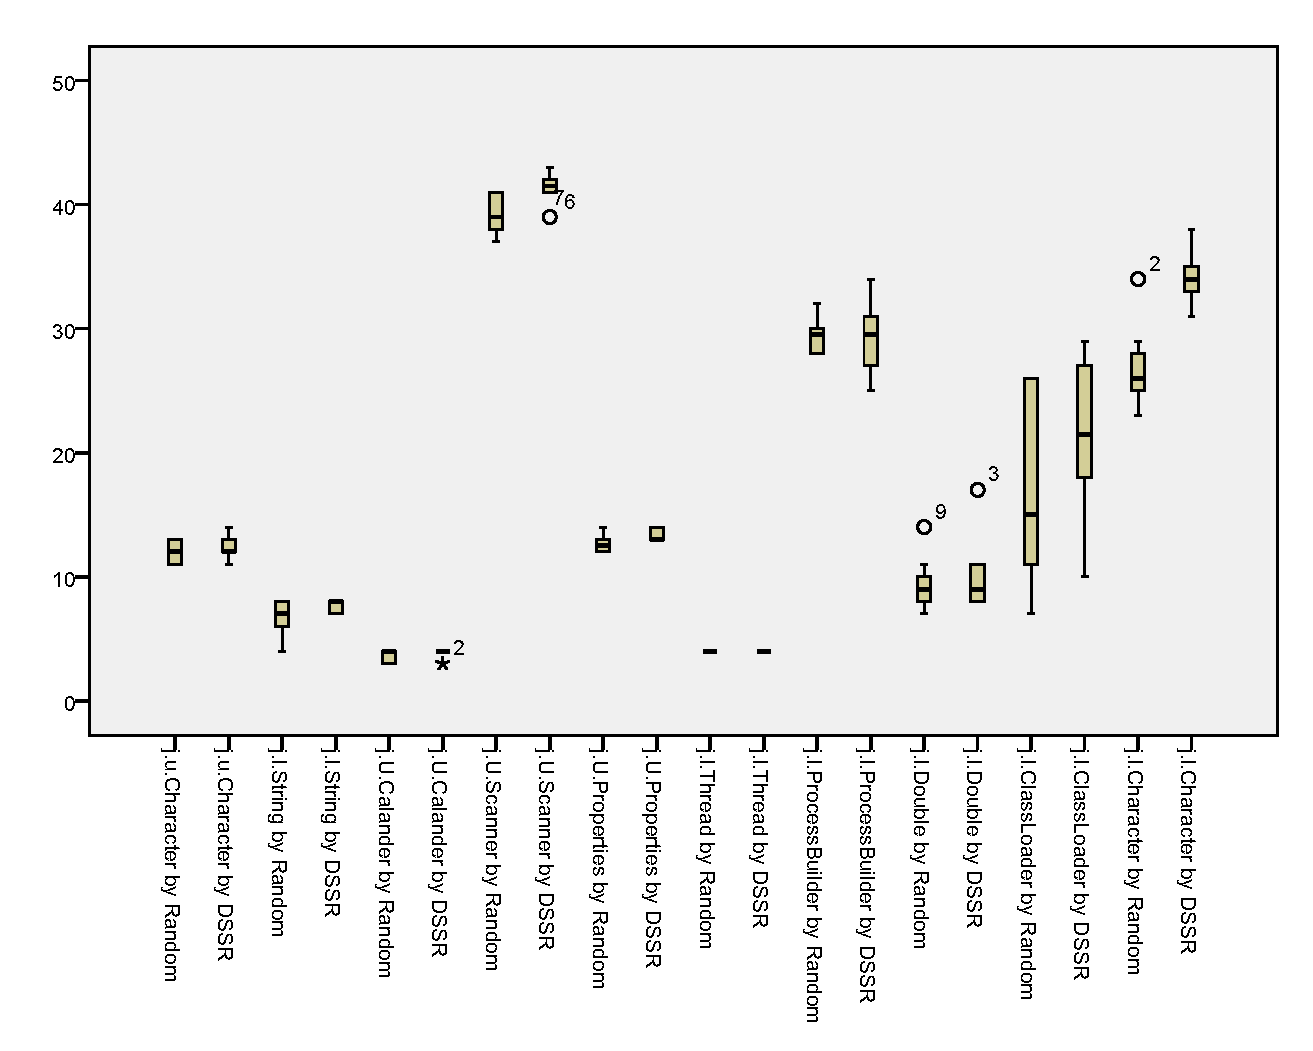
\includegraphics[width=8.5cm,height=7cm]{figures/javatests.png}
\caption{Test Results of 10 classes from java.util and java.lang package.}
\label{fig:Result2}
\end{figure}


%\pagenumbering{arabic}
%\setcounter{page}{1}

\section{Unique faults found by DSSR strategy}
Table \ref{table:DSS_Faults} include names of all the faults that DSSR strategy found in respective classes. Duplicate faults were removed for simplicity.

\begin{table}[ht]
\caption{Unique faults found by DSS in respective class} % title of Table
\centering % used for centering table
\begin{tabular}{| l | l |} % centered columns (4 columns)
\hline\hline %inserts double horizontal lines
Class Name & Unique Fault Name \\ [0.5ex] % inserts table
%heading
\hline % inserts single horizontal line
\multirow{3}{*}{java.lang.ProcessBuilder} & NullPointerException\\ % inserting body of the table
& YetiSecurityException\\ % inserting body of the table
& ArrayIndexOutOfBoundsException\\ % inserting body of the table
\hline
\multirow{2}{*}{java.lang.ClassLoader} & NoClassDefFoundError\\ % inserting body of the table
& IndexOutOfBoundsException\\ % inserting body of the table
\hline
\multirow{3}{*}{java.lang.Character} & StringIndexOutOfBoundsException\\ % inserting body of the table
& ArrayIndexOutOfBoundsException\\ % inserting body of the table
& IllegalArgumentException\\ % inserting body of the table
\hline
\multirow{7}{*}{java.util.Scanner} & IllegalArgumentException\\ % inserting body of the table
& NoSuchElementException\\ % inserting body of the table
& PatternSyntaxException\\ % inserting body of the table
& IllegalStateException\\ % inserting body of the table
& StringIndexOutOfBoundsException\\ % inserting body of the table
& InputMismatchException\\ % inserting body of the table
& UnsupportedOperationException\\ % inserting body of the table
\hline
\multirow{2}{*}{java.util.Properties} & NullPointerException\\ % inserting body of the table
& ClassCastException\\ % inserting body of the table
\hline
\multirow{2}{*}{java.util.Calendar} & ArrayIndexOutOfBoundsException\\ % inserting body of the table
& IllegalArgumentException\\ % inserting body of the table
\hline
java.lang.Double & NullPointerException\\ % inserting body of the table
\hline
\multirow{3}{*}{java.lang.Thread} & IllegalArgumentException\\ % inserting body of the table
& IllegalThreadStateException\\ % inserting body of the table
& NoSuchMethodError\\ % inserting body of the table
\hline
\multirow{4}{*}{java.lang.String}& PatternSyntaxException\\ % inserting body of the table
& IndexOutOfBoundsException\\ % inserting body of the table
& StringIndexOutOfBoundsException\\% inserting body of the table % [1ex] adds vertical space
\hline
\multirow{5}{*}{java.lang.Collections}& ClassCasteException\\ % inserting body of the table
& IndexOutOfBoundsException\\ % inserting body of the table
& UnsupportedOperationException\\
& IllegalArgumentException\\
& OutOfMemoryError\\ [1ex]% inserting body of the table % [1ex] adds vertical space
\hline
\hline %inserts single line
\end{tabular}
\label{table:DSS_Faults} % is used to refer this table in the text
\end{table}


\section{Discussion}

\textbf{Performance of DSSR strategy, Random strategy and Random plus strategy in terms of finding faults:} 
Analysis of results revealed that DSSR performs better than random and random plus in programs with block and strip pattern of faults. However, since not all the programs contain faults in the form of block and strip patterns therefore the overall results show that random plus strategy stood first, DSSR strategy second and pure random strategy comes third in finding faults. \\

\textbf{Time taken by DSSR strategy, Random strategy and Random plus strategy to execute tests:}
To execute equal number of test cases, DSSR strategy took slightly more execution time than pure random and random plus test strategy. It is not unusual and we were expecting similar behaviour because pure random algorithm selects random input of the required type with minimum calculation and therefore its process is very quick. On the other hand random plus and DSSR strategy performs additional computation when it maintains the list of interesting values and selects the correct type test values from the list when required. The desired process of adding values to the list and selecting the required values from the list consumes extra time which is the main reason that random plus and DSSR strategy takes a little extra time. Thus in executing tests random strategy, DSSR strategy and random plus strategy comes first, second and third respectively. \\

\textbf{Effect of test duration in terms of time and number of tests on test results:} 
We found that test duration increases either because of  increase in time or number of test cases which results in improving the performance of DSSR strategy than random and random plus. It is because when test duration or number of tests increases, the list of interesting values also increases and in turn DSSR strategy get enough relevant values in the list of interesting values and can easily pick one from the list instead of selecting it randomly or from static list of random plus.\\

\textbf{Effect of number of faults on results:} 
We also found that DSSR strategy performs better when the number of faults are more in the code. The reason is that when a fault is found in the code, DSSR strategy adds the neighbouring values of the fault finding value to the list of interesting values. Doing this increases the list of interesting values and the strategy is provided with more relevant test data resulting in higher chance of finding faults.\\

\textbf{Can Pure Random Testing perform better than DSSR strategy:}
The experimental results indicated that ocassionally pure random testing performs better than DSSR strategy if the SUT contain point pattern of failures rather than block and strip pattern. It is due to the fact that in such cases faults don't lay in the neighbourhood of found fault and adding neighbouring values of the founded fault dont make any impact on performance therefore the extra computational time becomes a liability.\\

\textbf{DSSR strategy Dependance on Random Testing:}
During the experiments we found that if the fault finding value is not in the list of interesting values then the test is dependant on random testing. In that case DSSR strategy has to wait for random testing to find the first fault and only then DSSR strategy will add its neighbouring values to the list of interesting values.

\section{Conclusion}

The main goal of the present study was to develop a new random strategy which could find more faults in lower number of test cases and shorter execution time. The experimental findings revealed that DSSR strategy was up to 30\% more effective in finding faults as compared to random test strategy. The DSSR strategy not only gave more consistent results but it proved more effective in terms of detecting faults as compared to random testing. However in comparison to random plus strategy both perform equally well in 95% of the experiments but in 5% random plus perform better and faster then DSSR strategy which is due to the fact that programs contain errors in the form of point patterns and adding fault neighbouring values only increases processing without improving results. \\

Improvement in performance of DSSR strategy over random strategy was achieved by taking advantage of Random Plus and fault neighbouring values. Random plus incorporated not only border values but it also added values having higher chances of finding faults in the SUT to the list of interesting values.\\

The DSSR strategy is highly effective in case of systems containing block and strip pattern of failure across the input domain.\\

Due to the additional steps of scanning the list of interesting values for better test values and addition of fault finding test value and its neighbour values, the DSSR strategy takes upto 5\% more time to execute equal number of test cases than pure random testing and 3% more than random plus. \\

In the current version of DSSR strategy, it might depend on random or random plus strategy for finding the first fault if the fault test value was not in the list of interesting values. Once the first fault is found only then DSSR strategy could make an impact on the performance of test strategy.\\

The limitation of random plus strategy is that it maintains a static list of interesting values which remains the same for each program under test, and can be effective in many cases but not always. The better approach will be to have a dynamic list of interesting values that is automatically updated for every program which can be achieved by adding the program literals and its surrounding values to the list of interesting values prior to starting every new test session.





\section{Future Work}

From the research we came to know that random testing is not very good in generating a specific test value as in the following example.  \\

\{ \\*   

\hspace{07 mm}if(value == 34.4445) \\*

\hspace{07 mm}\{ 10/0 \} \\* 

\} \\*


We also know that if the fault finding value is not in the list than DSSR has to wait for random testing to generate the fault finding value and only after that DSSR will add that value and its surrounding values to the list of interesting values. To decrease the dependancy of DSSR strategy on random and random plus strategy, further work is in progress to add constant literals from the SUT to the list of interesting values in a dynamic fashion. These literals can be obtained either from .java or .class files of the tested class. We are also working to add  neighbouring values of the literals to the list of interesting values. \\

Thus if we have the above example then the value 34.4445 and its surrounding values will be added to the list of interesting values before the test starts and DSSR strategy will no more be dependent on random testing to find the first fault.\\

It will also be interesting to evaluate the DSSR strategy in terms of coverage because the newly added values are most suitable for test cases and therefore can increase branch coverage. \\

Fianally, a significant part of our efforts is devoted to the evaluation of DSSR strategy by testing systems of different nature. We are planning to test up to 1000 classes from more than 100 open source Java projects of Qualitas Corpus, an independent database of open source Java project \cite{Tempero2010}. \\

% use section* for acknowledgement
\section*{Acknowledgment}
The auther would like to acknowldge with thanks the Department of Computer Science, University of York for the financial support extended as Departmental Overseas Research Scholarship (DORS) which enabled him to continue higher studies leading to PhD. We extend our sincere thanks and appreciation to Prof. Richard Page, Head of the Enterprise System's group of the Department of Computer Science for his valuable help and generous support.\\


\bibliographystyle{ieeetr}
\bibliography{biblio} 


% that's all folks
\end{document}


